\chapter{2}



Der ansteigende Schotterweg hinauf zum Felsen hatte sich über die Jahre
mit dem Gefühl freudiger Erwartung verbunden. Nach Freundschaft. Nach
Abenteuer auch.

Im gedeckten Abendlicht sah er schliesslich aus weiter Entfernung die
versammelte Gruppe Menschen. Die Szene wirkte vertraut, fast schon
familiär. Ein hohes Feuer gehörte längst dazu. Wie leicht es aussah.
Seine Leute, eingebettet in dieses kleine Stück Welt. Hier zwischen
uraltem Gestein und breitstämmigen Bäumen, in dieser weichen, schon fast
herbstlichen Dämmerung. Durchzogen vom Duft verbrannten Holzes stand die
Luft still, und eine erste Laubdecke hatte sich bereits lose unter die
einzelnen Baumgruppen gelegt.

Nach und nach drangen bekannte Stimmen zu ihm durch, gelegentlich
überlagert von ausgelassenem Gelächter. Ein friedvolles Bild als harter
Gegensatz zu Louis’ Stimmung.

Beim letzten Mal hier oben hatte er noch gehofft.

\sectionbreak

Bald waren einige Gestalten klar zu erkennen. Louis verlangsamte seinen
Schritt.

Dann sah er ihn. Als Ersten. Bastiano. Seine Bewegungen verrieten ihn.

Im Innersten bewunderte er Bastianos Gelassenheit. Gleichzeitig war da
Louis’ Zorn. Die Sicherheit, mit der er sich gab, liess Louis regelrecht
einknicken. Bastiano hatte etwas Einnehmendes. Louis wusste, er war
Giorgias bester Freund aus Kindertagen.

Auf Louis’ Frage, wie sie denn zu ihm stehe, hatte sie damals weit
ausgeholt.

\sectionbreak

Ins Geld geboren, hatte sie erzählt, wurden Bastiano schon als Kind
materielle Wünsche erfüllt, bevor er sie kannte. Seine Eltern waren
Grössen in Milano, angesehene, wohlhabende Leute. Rundum engagiert.

Bastiano hatte Tage, manchmal Wochen bei Giorgias Familie verbracht. Er
war auch ein Stück weit in der \emph{«Scuola di Danza»} gross geworden
und jeweils während des Sommers zum zweiten Kind der Familie Sala
geworden. Wie hatten sie die Wochen am Meer geliebt, hatte Giorgia
geschwärmt, waren unbekümmert und frei zwischen dem kleinen Haus am Meer
und dem Strand hin und her gependelt.

Louis konnte beobachten, wie nun ein wohliger Ruck durch Giorgia ging.

«Das war unsere, wie soll ich sagen, unsere goldene Zeit zusammen. Die
hat uns beide verbunden. Wir waren über die Jahre zu eingeschworenen
«Geschwistern» geworden.»

Es schwang auch ein bisschen Melancholie mit, glaubte Louis
herauszuhören.

Bastianos Wildheit, seine Abenteuerlust und die daraus gewachsenen,
grenzwertigen Katastrophen, hatten die kleine Giorgia fasziniert,
erklärte sie. Sie war zu seinem Anker geworden, hatte sich bei Bedarf
vor ihn gestellt. Und die Dinge wieder zurecht gerückt.

Bis Bastiano für mehrere Jahre verschwunden war. In ein Internat in den
Bergen, irgendwo in der Schweiz. Nur die nächsten Verwandten der Familie
durften wissen, dass Bastianos Eltern schon länger nicht mehr mit ihrem
Sohn zurechtkamen. Dass sie in Sorge waren vor einem Absturz ihres
Kindes. Sich davor fürchteten, ihr 14-jähriger, pubertierender und
einziger Sohn könnte ihnen entgleiten. Die Entscheidung war wohl viel
mehr Selbstschutz als wirkliche Problemlösung gewesen. Ein Akt der
Verzweiflung, wie Giorgia vermutete.

Sie hatte ohne Vorwarnung ihren «Bruder» verloren. Sei wochenlang
untröstlich gewesen. Bis sie ihm, dem 19-jährigen, Jahre später, wieder
begegnet war.

Giorgia sah bedrückt aus, während sie weitererzählte.

«Unser Wiedersehen war beklemmend. Wir wussten beide erstmal nichts zu
sagen. Es hat viel Zeit gebraucht, bis wir uns wieder nah waren. Er war
anders geworden, auch mir gegenüber.»

Sie stockte, suchte nach Worten.

Louis fühlte sich schon damals hin und her geworfen. Einerseits wollte
er alles wissen. Andererseits beklemmte ihn Giorgias leidenschaftliche
Art, ihm ihre Beziehung zu Bastiano zu schildern. Ihre Nähe zu ihm war
offensichtlich.

Giorgia hatte ihren Blick nachdenklich in die Ferne gerichtet. Und Louis
erinnerte sich, wie sie gedankenverloren ihren rechten Zeigefinger
mehrmals und rasch durch die Flamme der Kerze gezogen hatte, die auf dem
kleinen Tisch in der Küche stand.

«Er, er wirkte sicherer, auf eine mir fremde Art, und auch kalt,
manchmal.»

Sie schüttelte den Kopf, als wolle sie das Thema abschliessen. Lachte
unerwartet und stand mit einem Sprung auf.

«Aber dann fanden wir wieder zueinander. Wie Geschwister eben, die
zusammen aufgewachsen sind und die Geheimnisse voneinander kennen.»

\begin{center}
\vspace{0.8\baselineskip}
\begin{minipage}{\linewidth}
\centering
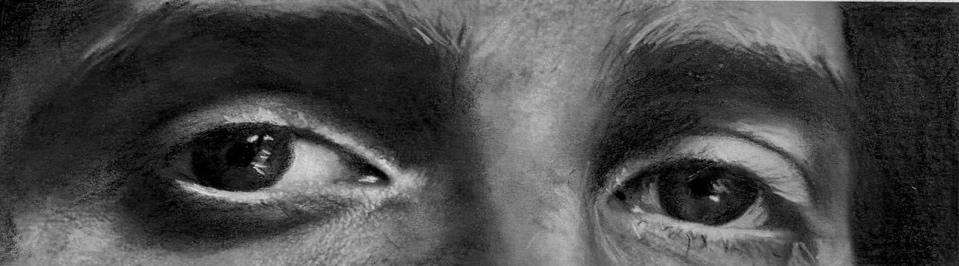
\includegraphics[width=\linewidth,height=!]{media/people/Bastiano.jpeg}
\par
\raggedright\textit{Bastiano Gabriele di Martino}
\end{minipage}
\vspace{0.3\baselineskip}
\end{center}

Eigentlich hatte Louis Giorgias Vertrautheit mit Bastiano von Anfang an
gestört. Zuerst nur leicht. Mit den Jahren zunehmend. Ihm war, als würde
der dauernd auftauchen, gelegentlich selbst dann, wenn sie zusammen
zuhause waren. Mit einer Selbstverständlichkeit, die Louis wunderte,
bald ärgerte und Giorgia zuliess.

Nichts davon hatte er je zu Giorgia gesagt. Wenn er knapp davorstand,
ihr Fragen zu stellen, verliess ihn der Mut. Und schliesslich, dachte er
sich, war es eine Frage der Ehre, wieviel Unsicherheit er Giorgia
gegenüber offenbarte.

Unverblümt, an einem Abend, hatte sie ihn genervt angesehen.

«Warum rivalisierst du mit Bastiano um mich? Was soll das?»

Giorgias Direktheit hatte Louis erschüttert. War einer Demaskierung
gleichgekommen. Er stand da, mit dem Rücken zur Wand. Wie ein
eifersüchtiger Trottel. Stumm suchte er hektisch nach Worten, die
schliesslich nicht zusammenpassten. Und hatte sie mit ihren Fragen
stehen lassen.

\sectionbreak

Giorgia hatte recht. Es hatte keine Chance für sie gegeben, zu ihm
durchzudringen. In diesen Momenten, wenn es darum ging, Schwächen zu
offenbaren. Die schweren, gut getarnten Türen zu seiner Welt der
unangenehmen Gefühle zu entriegeln. Giorgia Einlass zu gewähren in seine
ganz persönlichen Tiefen. Sie war die erste, die mehr von ihm wollte.
Die sich für Louis \emph{hinter} dem smarten Mann, dem
leidenschaftlichen Musiker, dem Freund, hinter dem kreativen Koch,
interessierte.

Die beiden ersten gemeinsamen Jahre hatten sich abenteuerlich und leicht
angefühlt. Der Alltag erst hatte ihre Unterschiede aufgedeckt. Sich
widersprechende Lebensweisen, Ansichten auch. Und Louis hatte sich immer
wieder gefragt, ob es darum ging, die Widersprüche auszuhalten oder sie
zu überwinden. Schwierige Situationen zu umschiffen war ihm vertrauter
geworden, als Zugeständnisse zu machen. Und dann hatte er es verpasst,
im richtigen Moment die Beziehung zu beenden. Wie er es mit seinen
Freundinnen vor Giorgia getan hatte. Bevor es unübersichtlich wurde und
er die Kontrolle verlor.

Seine Ahnung, Giorgia nicht mehr zu genügen, hatte sich über die Zeit
bewahrheitet. Mit jedem ihrer Konflikte war ihm klarer geworden, wie es
anders hätte sein müssen. Oder zumindest hätte werden sollen.

Dann war es zu spät gewesen.

\sectionbreak

«Louis?»

Er zuckte zusammen und drehte sich um.

«Warte!»

Valentina holte ihn mit kurzen Schritten ein.

«Hey, schön kommst du auch, trotz allem.»

Sie lächelte unsicher. Ihre Worte klangen wohlwollend. Und zugleich
mitleidig.

Sie wusste es. Alle wussten es.

Genau sieben Wochen waren seit dem 3. Juli vergangen. Valentinas
Bemerkung beschämte ihn. Ein Gefühl von Wertlosigkeit kam hoch.

«Ja.»

Er nickte und rang sich ein Lächeln ab.

Valentina umarmte Louis kurz und hakte sich bei ihm unter. Ihre Hand auf
seinem Arm fühlte sich beruhigend an.

In der Ferne sah er Franco aufstehen und ihnen entgegenkommen. Maria
folgte ihm. Franco wirkte vorsichtig. Als halte er seinen Frohmut in
Schach. Maria küsste Louis auf beide Wangen.

«Ich freue mich, dass du da bist. Wie geht es dir?»

Louis schluckte. In der Rolle des Leidenden hatte er im Kreis seiner
Leute wenig Übung.

«Geht so. Ich brauche wieder einmal das \emph{Roccia}-Feeling und euch.»

Louis’ Mund lächelte.

«Ach, Louis, und wir dich,» damit legte Franco ihm den Arm um die
Schulter. Zu viert näherten sie sich dem Feuerplatz. Die Grussworte von
rechts und links freuten Louis. Und für einen Moment war es ein bisschen
wie immer.

Bis er Giorgia sah, die sich gerade zwischen Bastiano und einem ihm
Unbekannten auf einen bankähnlichen, breiten Gesteinsblock setzte. Wie
schön sie anzusehen war.

Der Druck auf Louis’ Herz wuchs, je mehr sich die Distanz zu ihr
verringerte. Sie alle wirkten heiter. Er passte nicht dazu. Wie hatte er
nur nüchtern hier her kommen können. Ihm war, als falle er auseinander.

\sectionbreak

\emph{Damals. Fribourg, fünf.}

\emph{Louis sitzt am Küchentisch. Vor ihm das neue Lernbuch. Maman hat es ihm
gekauft. Seine Hand führt den Bleistift den schmalen Weg entlang von der
Katze bis zur Maus. Er liebt es, Labyrinthe zu entschlüsseln. Wie aus
dem Nichts steht sein Vater vor ihm. Von weit oben schaut er auf ihn
hinunter.}

\emph{«Gut machst du das, mein Sohn, du bist der Beste und bestimmt der
Klügste in deinem Kindergarten. Dich kann keiner erreichen.»}

\emph{Vater lacht, tätschelt ihm die Wange und Louis wartet. Es kommt.}

\emph{«Wir sind die Grössten. Wir zwei.»}

\emph{Warum Maman nur jedes Mal den Kopf schüttelt? Ein warmes Gefühl
durchströmt ihn. Er hört die Worte immer wieder. Es beschwingt ihn,
seinem Vater gleich zu sein.}

\emph{In null Komma nichts löst er die Aufgabe. Er ist stolz. Will sein Werk
zeigen. Vater steht unterdessen abseits. Er ist am Telefon und winkt ab.
Jetzt hat er keine Zeit mehr. Louis ist enttäuscht und fragt sich, wozu
er das Rätsel gelöst hat.}

\sectionbreak

Er hatte keine Wahl gehabt, damals, Vater nicht zu glauben.

Die Überzeugung hielt sich. Erst nach Jahren hatte sie begonnen,
abzublättern. Hatten sich Wirkungslosigkeit und Lächerlichkeit seines
kindlichen Glaubens an diese eigene Herrlichkeit gegenseitig zu
überbieten begonnen.

Dennoch \emph{«Du bist der Beste!»} hatte sich als Leitsatz über die
Jahre eingeimpft und gehalten. Und schliesslich als Belastung quer über
seiner Brust installiert. Mit massiger Schwere. War aufsässig geblieben
und suchte unentwegt nach Bestätigung.

Louis versuchte, die Erinnerung von sich zu stossen. Dahin zurück, wo
sie hergekommen war.

\sectionbreak

Bald war es unausweichlich, dass die Klänge ihn trafen. Scharf wie
hauchdünne Blechkanten. Luis Fonsis \emph{«Despacito»} ergoss sich
über die tanzende Gruppe. Alle lachten. Louis nicht.

Augenblicklich war dieser weit zurückliegende Abend präsent. Wie nah
Giorgia und er sich letzten Sommer noch gewesen waren, oder jedenfalls
immer mal wieder.

Giorgia hatte Louis zugezwinkert, während «Despacito» lief.

«Ich stell mir vor, \emph{du} singst für mich,» sie schloss die Augen,
demonstrativ angestrengt und klang fröhlich, «denselben Namen habt ihr
schon mal, das kann ja kein Zufall sein.»

Und Louis hatte sie gehalten, war verrückt gewesen nach ihr. Und hatte
es genossen. Giorgia war anders als alle Frauen.

\qrblock{Luis Fonsi and Daddy Yankee \emph{«Despacito»}}{media/QR-Codes/008_Despasito_Luis_Fonsi,_Daddy_Yankee_Spotify.png}

Es war geradezu niederträchtig. Der \emph{«Roccia del Culto»} hatte sich
für Louis zum Monster entwickelt. \emph{«Fels der Anbetung!»} -- dass er
nicht lachte. Damals hatte er es euphorisch als Prophezeiung gesehen.
Sie waren das erste Mal eng umschlungen den Hügel hinauf geschlendert.
Giorgia gehörte zu ihm.

Nunmehr ein einziger Hohn.

\sectionbreak

Was hatte Giorgias Trennung nur mit ihm angestellt. Ihre Abweisung war
nichts anderes als eine respektlose Erniedrigung. Als hätte sie ihn vor
versammelter Menge geohrfeigt. Der Gedanke war unerträglich. Kurz
stellte sich wieder diese Kraft ein, die ihn in Momenten der Traurigkeit
aus seiner Lethargie hob. Er sollte verschwinden. Doch die Kraft ging,
wie gekommen. Er fühlte sich starr wie eine Statue.
